% =====================================================================
%  ch08.tex —— 第 8 章 Chern–Simons 项（原书 p.118–128）
%  §8.1 电荷的量子化  §8.2 霍尔电导的量子化  §8.3 评注
%  注意：p.118 上半页属第 7 章末尾（§7.5.3 分类空间与示性类，式 (7.69)–(7.71)），
%        按整页切块归入本 chunk。故本文件依次为：§7.5.3 正文、§7.5 的 takeaway、
%        第 7 章的 chapterreview、再 \chapter{Chern--Simons 项}，与原书版式一致。
% =====================================================================

% [原文 p.118]
\subsection{分类空间与示性类}

分类空间为理解示性类提供了统一的途径；此前这些类都是逐个情形构造的。
设给定主 $G$ 丛 $G\to P\to X$。相应地有映射 $f_P:X\to BG$。
现在取上同调类 $a\in H^k(BG;A)$，把它拉回到 $X$，得到 $f_P^*(a)\in H^k(X;A)$。
这样，就由给定的主 $G$ 丛构造出了 $H^k(X;A)$ 中的一个上同调类。

例如取 $G=U(1)$。则 $H^2(BU(1);\Z)=H^2(\CP^\infty;\Z)=\Z$。
记其生成元为 $c_1$。于是对任意主 $U(1)$ 丛 $U(1)\to P\to X$，有映射 $f_P:X\to BU(1)$。
拉回得到上同调类 $f_P^*(c)\in H^2(X;\Z)$。可以把它与丛 $P$ 的第 1 Chern 类 $c_1(P)$ 等同，即
\begin{equation}
f_P^*(c_1)=c_1(P).
\tag{7.69}
\end{equation}

类似地，对 $G=SO(3)$，有 $H^2(BSO(3);\Z_2)=\Z_2$，记其生成元为 $w_2$。
于是对任意主 $SO(3)$ 丛 $SO(3)\to P\to X$，有映射 $f_P:X\to BSO(3)$。
拉回 $w_2$ 得上同调类 $f_P^*(w_2)\in H^2(X;\Z_2)$。
这就是丛 $P$ 的第 2 Stiefel--Whitney 类 $w_2(P)$，即
\begin{equation}
f_P^*(w_2)=w_2(P).
\tag{7.70}
\end{equation}
类似地，有类 $W_3\in H^3(BSO(3);\Z)$，并且
\begin{equation}
f_P^*(W_3)=W_3(P).
\tag{7.71}
\end{equation}

从这个观点看，要确定主 $G$ 丛所有可能的示性类，只需研究各种系数 $A$ 下的 $H^*(BG;A)$。
于是示性类的分类，就化归为分类空间上同调群的研究。

\takeaway{分类空间 $BG$ 使主 $G$-丛的同构类与映射 $X\to BG$ 的同伦类一一对应；示性类就是从 $BG$ 的上同调拉回得到的类，$K(A,k)$ 空间同理分类上同调类。}

\chapterreview{本章以 Čech 上同调逐级构造示性类。次数 1：有限阿贝尔群 $A$ 的主丛给出 $H^1(M;A)$ 中的类，配对是绕闭链的和乐；用行列式得第 1 Stiefel--Whitney 类 $w_1$，它衡量丛能否约化为 $SO(n)$。次数 2：$U(1)$ 丛的粘贴函数写成指数，在三重交上留下整数 2-上闭链，得第 1 Chern 类 $c_1$，即曲率积分；对 $SO(3)$ 丛类似得 $w_2$，衡量能否提升为 $SU(2)$ 或 $Spin(n)$ 丛。次数 3：把模 2 约化提升为整数上链，其失效给出 Bockstein 同态 $\beta$，$\beta(w_2)$ 是提升为 $U(2)$ 丛的障碍。分类空间则把这一切统一为 $BG$ 的上同调。}

\chapter{Chern--Simons 项}

\section{电荷的量子化}

上面我们看到，$U(1)$ 丛的数学性质自然导致磁荷的 Dirac 量子化。
那电荷的量子化又该怎么理解？理解的方式取决于你取粒子观点还是波观点。

\subsection{波的观点}

在波的观点下，给定时空 $M$ 上的 $U(1)$ 丛 $P\to M$，
带电场是某个相伴复线丛 $L\to M$ 的截面。更具体地说，
若两个覆盖块 $U$ 与 $U'$ 之间的 $U(1)$ 丛由下式给出：
\begin{equation}
U\times U(1)\supset(U\cap U')\times U(1)\ni(x,z)\mapsto(x,gz)
\in(U\cap U')\times U(1)\subset U'\times U(1),
\tag{8.1}
\end{equation}

% [原文 p.119]
其中 $g:U\cap U'\to U(1)=\{g\in\C\mid|g|=1\}$，则允许的复线丛按如下规则粘贴：
\begin{equation}
U\times\C\supset(U\cap U')\times\C\ni(x,v)\mapsto(x,g^nv)
\in(U\cap U')\times\C\subset U'\times\C.
\tag{8.2}
\end{equation}
这里 $g^n$ 必须是良定义的函数，因此 $n$ 必须是整数。

设 $(x,\psi(x))$ 是这个线丛的截面。则 §5.5 讨论过的协变导数变为
\begin{equation}
D\psi:=\sum_a\left(\frac{\partial}{\partial x^a}-inA_a\right)\psi dx^a.
\tag{8.3}
\end{equation}
这里的系数 $n$ 意味着 Maxwell 场 $A$ 与带电场 $\psi$ 的耦合正比于 $n$，
即电荷正比于 $n$。这是理解电荷量子化的一条途径。

\subsection{从粒子观点看（第一部分）}

改用粒子观点。质量为 $m$、电荷为 $q$ 的带电非相对论粒子的经典作用量为
\begin{equation}
S=\int\left(\frac m2|v|^2+q^{\text{SI}}\Bigl(A_t^{\text{SI}}
+\sum_aA_a^{\text{SI}}v^a\Bigr)\right)dt,
\tag{8.4}
\end{equation}
其中 $v^a=dx^a/dt$。等价地有
\begin{equation}
S=\int\frac m2|v|^2dt+q^{\text{SI}}\int A^{\text{SI}},
\tag{8.5}
\end{equation}
其中 $A^{\text{SI}}$ 现在被看作 1-形式，$\int A^{\text{SI}}$ 是其积分。
这并不完全妥当，因为矢势 $A^{\text{SI}}$ 其实不是 1-形式。
但在经典力学里这不会造成问题。的确，在规范变换
\begin{equation}
A^{\text{SI}}\mapsto(A^{\text{SI}})' :=A^{\text{SI}}+d\chi
\tag{8.6}
\end{equation}
下，积分的变化为
\begin{equation}
\int_p^q(A^{\text{SI}})'-\int_p^qA^{\text{SI}}=\chi(q)-\chi(p),
\tag{8.7}
\end{equation}
只依赖边界值。这不影响作用量变分的计算。

然而在量子力学里这会带来问题。用路径积分表述，需要考虑
\begin{equation}
Z=\int\mathcal{D}x^a\exp\left(\frac{i}{\hbar}
\Bigl(\int_C\frac m2|v|^2dt+q^{\text{here}}\int_CA^{\text{geometric}}\Bigr)\right)
\tag{8.8}
\end{equation}

% [原文 p.120]
这里假设
\begin{equation}
A^{\text{geometric}}=kA^{\text{SI}},
\tag{8.9}
\end{equation}
其中 $k$ 是某个比例系数，于是
\begin{equation}
q^{\text{here}}=q^{\text{SI}}/k.
\tag{8.10}
\end{equation}
$A^{\text{geometric}}$ 的规范变换为
\begin{equation}
A^{\text{geometric}}\mapsto(A^{\text{geometric}})' := A^{\text{geometric}}+ig^{-1}dg,
\tag{8.11}
\end{equation}
其中 $g\in U(1)$。这意味着
\begin{equation}
\int_C(A^{\text{geometric}})'=\int_CA^{\text{geometric}}+2\pi w,
\tag{8.12}
\end{equation}
其中 $w\in\Z$ 是 $g:C\to U(1)$ 的缠绕数。这意味着指数的值会乘性地平移
\begin{equation}
\exp\Bigl(\frac{2\pi i}{\hbar}q^{\text{here}}w\Bigr),
\tag{8.13}
\end{equation}
其中 $w$ 是任意整数。这要求取 $q^{\text{here}}=\hbar n$（$n$ 为某整数），
即 $q^{\text{SI}}=k\hbar n$（$n$ 为某整数）。
这就使上面把比例系数取为 $k=e/\hbar$ 显得合理。

\subsection{从粒子观点看（第二部分）}

换一种稍有不同的方式，导出 $q^{\text{here}}$ 必须是整数，这种方式便于日后的推广。
当 $A^{\text{geometric}}$ 是 1-形式、且 $C$ 是圆盘的边界 $C=\partial D$ 时，由 Stokes 定理有
\begin{equation}
\int_CA^{\text{geometric}}=\int_DF^{\text{geometric}},
\tag{8.14}
\end{equation}
这里假定 Maxwell 场在 $D$ 上也有定义。虽然 $A^{\text{geometric}}$ 其实不是 1-形式，
但 $F^{\text{geometric}}$ 是真正的 1-形式。于是可以试着用右端来定义 (8.14) 的左端：
% [Tutor Note: 按通常约定 $F=dA$ 是 2-形式，此句原文作 1-form，疑为笔误；译文照录。]
\begin{equation}
\int_CA^{\text{geometric}}:=\int_DF^{\text{geometric}},
\tag{8.15}
\end{equation}
这适用于 $A^{\text{geometric}}$ 不完全是 1-形式的更一般情形。

右端总是良定义的，但引入了另一个问题：它不仅依赖 $C$ 上的规范配置，还依赖整个 $D$。
为研究这种依赖，设我们把 $C$ 上的规范配置以两种方式分别延拓到 $D$ 与 $D'$。
需要研究式 (8.14) 的右端在 $D$ 与 $D'$ 上的差：
\begin{equation}
\int_{D'}F^{\text{geometric}}-\int_DF^{\text{geometric}}
=\int_{D'\cup\bar D}F^{\text{geometric}},
\tag{8.16}
\end{equation}
见图 8.1。

% [原文 p.121]
\begin{center}
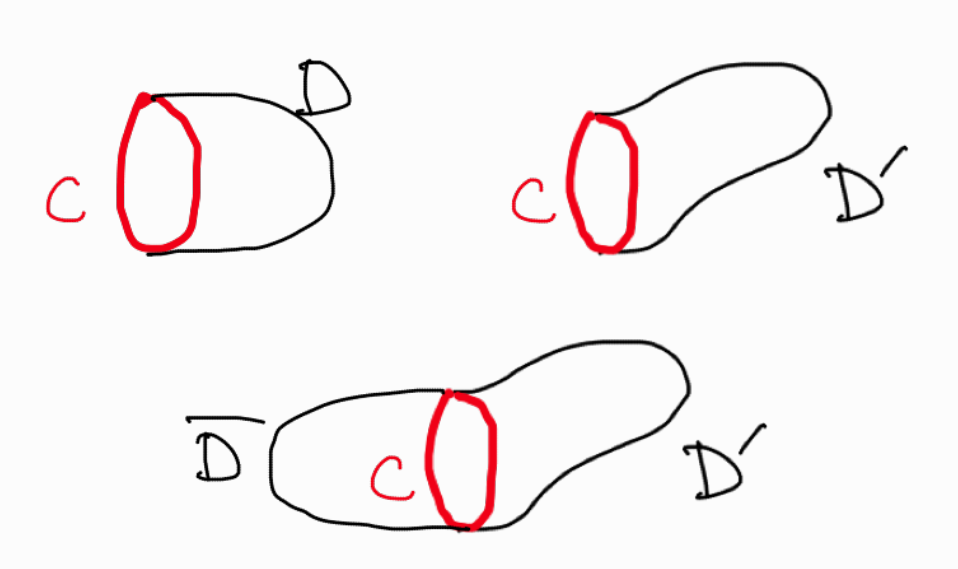
\includegraphics[width=0.62\textwidth]{figures/fig8_1.png}\\[2pt]
{\small 图 8.1：围道 $C$ 与辅助的包围曲面 $D$、$D'$}
\end{center}

我们知道，$F^{\text{geometric}}$ 在闭曲面上的积分量子化为 $2\pi w$，其中 $w$ 是某整数。
这意味着 $\int_DF^{\text{geometric}}$ 模 $2\pi w$ 不依赖 $D$ 上规范配置延拓方式的选取，因此
\begin{equation}
\exp\Bigl(in\int_CA^{\text{geometric}}\Bigr)
:=\exp\Bigl(in\int_DF^{\text{geometric}}\Bigr)
\tag{8.17}
\end{equation}
对任意整数 $n$ 都良定义。特别地，我们导出了 $q^{\text{here}}=\hbar n$，$n$ 为某整数。

\takeaway{电荷量子化来自两点：粘贴函数取 $n$ 次幂要求 $n$ 为整数；路径积分的相位必须良定义，迫使 $q=\hbar n$。$\int A$ 与 $\int A\wedge F$ 的歧义依次为 $2\pi$ 与 $(2\pi)^2$。}

\section{霍尔电导的量子化}

\subsection{物理背景}

在二维材料中，外加电压与电流的关系一般写成
\begin{equation}
\begin{pmatrix}I_x<本地路径>
=\begin{pmatrix}\sigma_{xx}&\sigma_{xy}\\ \sigma_{yx}&\sigma_{yy}\end{pmatrix}
\begin{pmatrix}V_x<本地路径>,
\tag{8.18}
\end{equation}
其中 $\sigma_{ij}$ 是电导张量的分量。在某种实验情形下 $\sigma_{xx}=\sigma_{yy}=0$，
霍尔电导 $\sigma_{xy}$ 量子化为 $e^2/h$ 的整数倍，
其中 $e$ 是基本电荷，$h$ 是 Planck 常数：
\begin{equation}
\sigma_{xy}=\nu\frac{e^2}{h}.
\tag{8.19}
\end{equation}
这称为整数量子霍尔效应。经典实验与较近的实验结果各一例，见图 8.2。

理解这一量子化现象有多种理论途径。这里想讨论一种教科书里通常不讲的做法。
我并不是说它比别的方法更好，只是别的方法在许多标准教科书里都有，
而这个方法与本讲义的内容非常契合。

% [原文 p.122]
\begin{center}
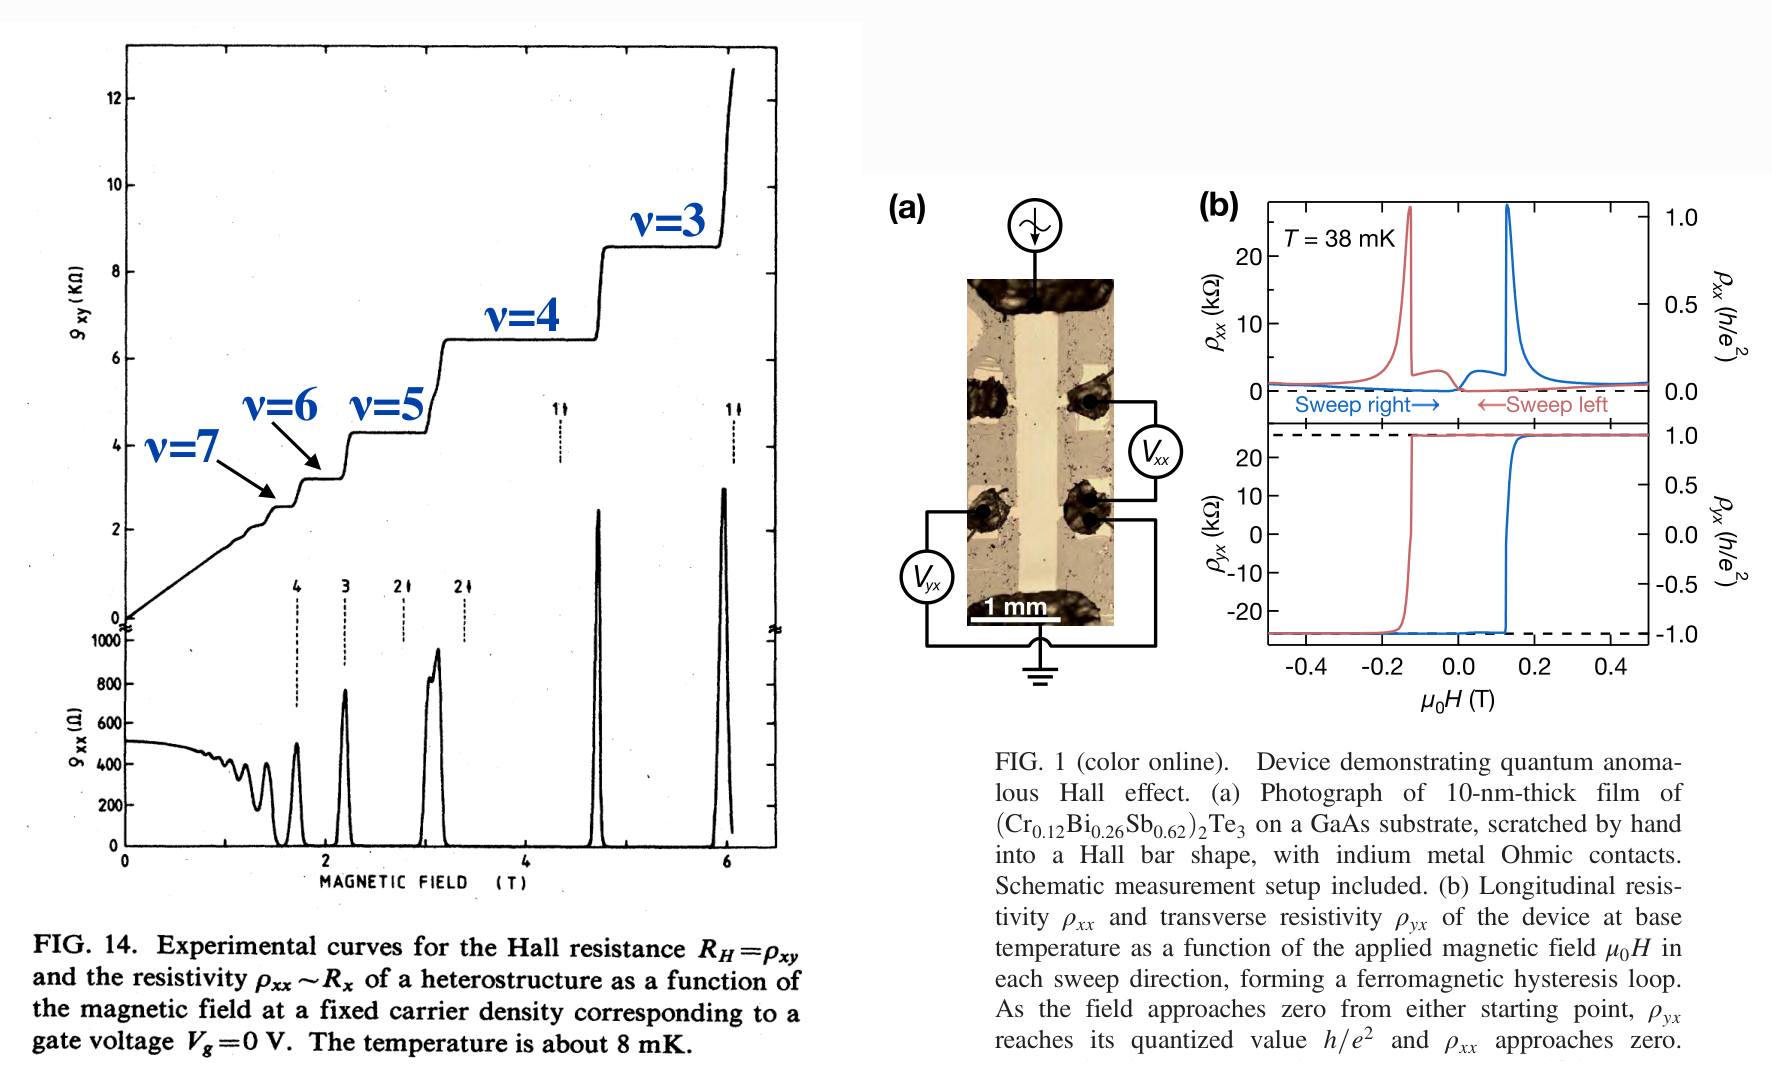
\includegraphics[width=0.92\textwidth]{figures/fig8_2.png}\\[2pt]
{\small 图 8.2：左：取自 von Klitzing 的经典综述 [vK86]；右：取自 2015 年的现代实验 [BFK+15]。}
\end{center}

% [原文 p.123]
有整数量子霍尔效应的一般情形，是系统有能隙，且在非平凡的空间流形（比如环面 $T^2$）上
基态唯一。相反，若系统有能隙，但在非平凡空间流形上有多个基态，
霍尔电导就不再量子化为整数，而是量子化为有理数。这就是分数量子霍尔效应。
最后，若系统没有能隙，霍尔电导不量子化。汇总见表 4。

\begin{center}
\begin{tabular}{ccc}
\toprule
有能隙？ & 基态数 & $\sigma_{xy}$ 的量子化\\
\midrule
是 & 唯一 & 整数\\
是 & 多重 & 有理数\\
否 & 不适用 & 不量子化\\
\bottomrule
\end{tabular}\\[2pt]
{\small 表 4：各种情形下霍尔电导的量子化}
\end{center}

\subsection{数学分析}

设系统有能隙，且基态唯一。设想把系统放到非平凡的三维流形 $M_3$ 上，
并加一个外 Maxwell 场 $P\to M_3$ 来探测其电学性质。
这在实验上是否可行无关紧要；要点只在于把系统放到这种非平凡流形上的可能性。
系统的配分函数 $Z$ 依赖 $M_3$ 与外 Maxwell 场 $P\to M_3$。
它由单个基态的贡献主导，因此只是一个相位：
\begin{equation}
Z(M_3,P)=\exp\bigl((i/\hbar)S(M_3,P)\bigr),
\tag{8.20}
\end{equation}
其中 $S(M_3,P)$ 应当是模整数良定义的实数。

若系统有能隙但有多个基态，$Z(M_3,P)$ 是各基态贡献之和，因此不能取成简单的相位。
若系统没有能隙，$Z(M_3,P)$ 还要更复杂。
看似简单的式 (8.20)，正是要从物理上导出霍尔电导整数量子化所需的关键输入。

注意，感生电流与电荷密度由 $S$ 对外 Maxwell 场的变分给出：
\begin{equation}
\delta S=\int_{M_3}\Bigl(\rho^{\text{SI}}\delta A_t^{\text{SI}}
+\sum_aj_a^{\text{SI}}\delta A_a^{\text{SI}}\Bigr)dtdxdy.
\tag{8.21}
\end{equation}

设霍尔电导 $\sigma^{\text{SI}}:=\sigma_{xy}$。
我们要 $j_x^{\text{SI}}=\sigma E_y^{\text{SI}}$ 与 $j_y^{\text{SI}}=-\sigma E_x^{\text{SI}}$。
简单计算给出
\begin{align}
S&=\frac{\sigma^{\text{SI}}}{2}\int_{M_3}
\bigl(A_t^{\text{SI}}F_{xy}^{\text{SI}}+A_x^{\text{SI}}F_{yt}^{\text{SI}}
+A_y^{\text{SI}}F_{tx}^{\text{SI}}\bigr)dtdxdy \tag{8.22}\\
&=\frac{\sigma^{\text{SI}}}{2}\int_{M_3}A^{\text{SI}}\wedge F^{\text{SI}} \tag{8.23}
\end{align}

% [原文 p.124]
当 $A$ 在 $M_3$ 上整体定义时，这个表达式正合要求。
因子 $1/2$ 来自这样一个事实：$\delta A$ 既来自 $A$ 的变分，也来自 $F$ 的变分。

但在更一般的情形，$A$ 不是整体定义的 1-形式，这个表达式就没有意义；
而 $\exp((i/\hbar)S)$ 却必须良定义。下面照旧进行。
暂时用 $A^{\text{geometric}}$ 代替 $A^{\text{SI}}$。
设 $M_3$ 是某个 $N_4$ 的边界，$M_3=\partial N_4$。于是当 $A^{\text{geometric}}$
是整体定义的 1-形式时，有
\begin{equation}
\int_{M_3}A^{\text{geometric}}\wedge F^{\text{geometric}}
=\int_{N_4}F^{\text{geometric}}\wedge F^{\text{geometric}}.
\tag{8.24}
\end{equation}
这促使我们用右端来定义左端：
\begin{equation}
\int_{M_3}A^{\text{geometric}}\wedge F^{\text{geometric}}
:=\int_{N_4}F^{\text{geometric}}\wedge F^{\text{geometric}}.
\tag{8.25}
\end{equation}

这个做法有两个问题：
\begin{itemize}
  \item 对给定的 $M_3$，是否存在合适的 $N_4$，并不清楚。同样不清楚的是：
        即使这样的 $N_4$ 存在，$M_3$ 上的 $U(1)$ 丛能否延拓到 $N_4$。这些是存在性问题。
        注意，此前讨论 $\int_CA$ 的类似定义时并没有这个问题，
        因为任何 $C=S^1$ 都能延拓为 $D^2$，$S^1$ 上任何 $U(1)$ 丛也都能延拓到其内部。
  \item 设合适的 $N_4$ 与 $U(1)$ 丛的延拓都存在，它们也并不唯一。
        而且右端不仅依赖 $M_3$ 上的规范配置，还依赖整个 $N_4$。
        因此不清楚它是否给出一个良定义的量。
\end{itemize}

遗憾的是，我们没有时间深入存在性问题。这可以用配边（bordism）理论研究。
在一般维数、一般 $G$-丛的情形，答案是否定的。所幸在这个时空维数下、对 $U(1)$ 丛，
答案却是肯定的。

为研究不唯一性带来的问题，考虑两个可能不同的 $N_4$ 与 $N_4'$，
以及 $U(1)$ 场配置的两种可能不同的延拓。于是有
\begin{equation}
\begin{split}
&\int_{N_4'}F^{\text{geometric}}\wedge F^{\text{geometric}}
-\int_{N_4}F^{\text{geometric}}\wedge F^{\text{geometric}}\\
&\qquad=\int_{W_4}F^{\text{geometric}}\wedge F^{\text{geometric}},
\end{split}
\tag{8.26}
\end{equation}
其中 $W_4=N_4'\cup\ol{N_4}$，见图 8.3。

现在注意，$[F^{\text{geometric}}/2\pi]$ 来自 $U(1)$ 丛 $P\to W_4$ 的第 1 Chern 类
$c_1(P)\in H^2(W_4;\Z)$，特别地
\begin{equation}
\frac{1}{(2\pi)^2}\int_{W_4}F^{\text{geometric}}\wedge F^{\text{geometric}}
=\langle c_1(P)\cup c_1(P),[W_4]\rangle\in\Z.
\tag{8.27}
\end{equation}

这意味着 (8.25) 的右端模 $(2\pi)^2$ 良定义，因此下面的表达式对整数 $n$ 良定义：
\begin{equation}
\exp\Bigl(i\frac{n}{2\pi}\int_{M_3}A^{\text{geometric}}\wedge F^{\text{geometric}}\Bigr)
=\exp\Bigl(\frac{i}{\hbar}\frac{ne^2}{h}\int_{M_4}A^{\text{SI}}\wedge F^{\text{SI}}\Bigr).
\tag{8.28}
\end{equation}

% [原文 p.125]
\begin{center}
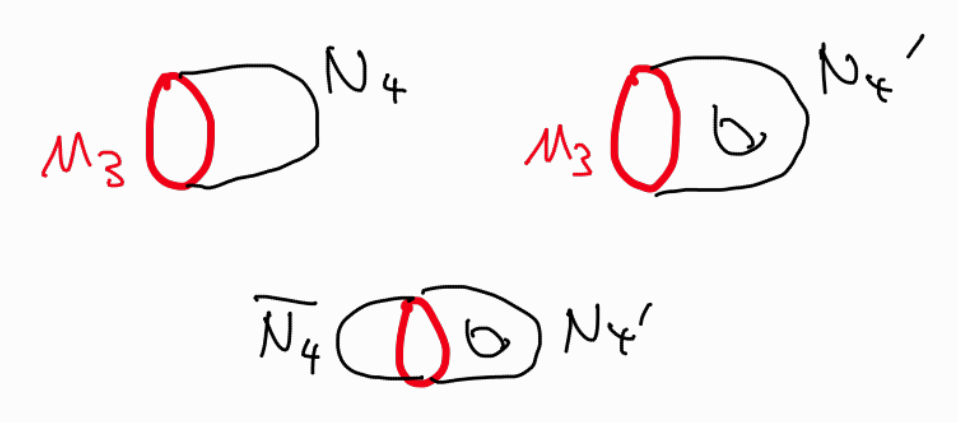
\includegraphics[width=0.62\textwidth]{figures/fig8_3.png}\\[2pt]
{\small 图 8.3：$M_3$ 作为边界，以及辅助的包围四维流形 $N_4$、$N_4'$}
\end{center}

与式 (8.23) 比较可知，这意味着配分函数 (8.20) 在
\begin{equation}
\sigma^{\text{SI}}=2n\frac{e^2}{h}
\tag{8.29}
\end{equation}
时良定义，其中 $n$ 为整数。这与通常的表达式 (8.19) 相差一个因子 2。

挽救局面的是下面这个数学定理：

\begin{theorem}{8.1}
在闭的 spin 四维流形 $W_4$ 上，对类 $a\in H^2(W_4;\Z)$，量
\begin{equation*}
\langle a\cup a,[W_4]\rangle
\end{equation*}
不仅是整数，而且是偶数。
\end{theorem}

现在我们要求涉及的所有流形 $M_3$、$N_4$、$N_4'$、$W_4$ 都是 spin 流形。
于是式 (8.25) 的右端模 $2(2\pi)^2$ 良定义，因此对任意整数 $\nu$，表达式
\begin{equation}
\exp\Bigl(i\frac{\nu}{2\cdot2\pi}\int_{M_3}A^{\text{geometric}}\wedge F^{\text{geometric}}\Bigr)
=\exp\Bigl(\frac{i}{\hbar}\frac{\nu e^2}{2h}\int_{M_4}A^{\text{SI}}\wedge F^{\text{SI}}\Bigr)
\tag{8.30}
\end{equation}
良定义。这意味着霍尔电导应当满足
\begin{equation}
\sigma^{\text{SI}}=\nu\frac{e^2}{h}.
\tag{8.31}
\end{equation}

这样就知道：$\nu$ 为奇数时霍尔电导的量子化，要求所涉流形上具有 spin 结构。
这在物理上完全合理，因为电子是自旋 $1/2$ 的粒子，要在流形上传播就需要 spin 结构。
它对整数量子霍尔效应量子化单位的影响，是这一物理要求相当间接却耐人寻味的推论。

\takeaway{有能隙且基态唯一时，配分函数只是相位 $e^{iS/\hbar}$。把系统放到三维流形上，$S$ 的良定义性迫使 $A\wedge F$ 的积分取整；差的因子 2 由 spin 四维流形上 $a\cup a$ 为偶数的定理补足，于是得到 $\sigma_{xy}=\nu e^2/h$。}

\section{评注}

本节以几点评注收尾。

% [原文 p.126]
\subsection{阿贝尔 Chern--Simons 项}

本节讨论了当 $A$ 不是整体定义的 1-形式时，如何定义 $\int_CA$ 与 $\int_{M_3}A\wedge F$。
我们看到：$\int_CA$ 可以做到模 $2\pi$ 良定义；$\int_{M_3}A\wedge F$
在可定向流形上可以做到模 $(2\pi)^2$ 良定义，在 spin 流形上可以做到模 $2(2\pi)^2$ 良定义。

在更高维，自然的推广是
\begin{equation}
\int_{M_{2n-1}}A\wedge F^{n-1},
\tag{8.32}
\end{equation}
它们称为（阿贝尔）Chern--Simons 项。这一项出现在理论物理的许多场合。
例如下一个版本 $\int_{M_5}AF^2$ 出现在四维手征费米子的微扰 $U(1)$ 反常的研究中。

利用 $F/2\pi$ 对应 $U(1)$ 丛的 $c_1$ 这一事实，容易把式 (8.32) 在可定向流形上
做到模 $(2\pi)^n$ 良定义。但我们已经看到，对霍尔电导 $n=2$ 的量子化来说这还不够。
同样，若想把 $n=3$ 的版本用于 $U(1)$ 反常的研究，也还不够。
粗略地说，已知 spin 结构能把定义从模 $(2\pi)^n$ 精化为模 $n!(2\pi)^n$。
但要解释这一点，所需时间比我们这里能给的要多得多。

\subsection{再论 $n=2$ 的情形}

在 $n=2$ 的情形，spin 结构使 $\int A\wedge F$ 的歧义从模 $(2\pi)^2$ 降到模 $2(2\pi)^2$。
这种把歧义减半的精细化的通称是二次精化（quadratic refinement）。
在我们的情形，它依赖作为定理 8.1 引用的那个数学事实。
下面通过说明这个定理如何证明，来展示其中牵涉到什么样的代数拓扑。

我们要证明：若 $W_4$ 是 spin 流形，则对 $a\in H^2(W_4;\Z)$，$\langle a\cup a,[W_4]\rangle$ 是偶数。
设 $\tilde a\in H^2(W_4;\Z_2)$ 是 $a$ 的模 2 约化。由于
\begin{equation}
\langle a\cup a,[W_4]\rangle=\langle\tilde a\cup\tilde a,[W_4]\rangle\mod 2,
\tag{8.33}
\end{equation}
只需证明
\begin{equation}
\langle\tilde a\cup\tilde a,[W_4]\rangle\equiv0\mod 2,
\tag{8.34}
\end{equation}
对 $W_4$ 为 spin 时的所有 $\tilde a\in H^2(W_4;\Z_2)$ 成立。

现在碰巧存在一个自然变换
\begin{equation}
Sq^k:H^n(M;\Z_2)\to H^{n+k}(M;\Z_2),
\tag{8.35}
\end{equation}
称为 Steenrod 平方，它满足
\begin{equation}
Sq^ka_k=a_k\cup a_k
\tag{8.36}
\end{equation}
其中 $a_k\in H^k(M;\Z_2)$。

% [原文 p.127]
设 $n$ 是 $M$ 的维数。取 $a_{n-k}\in H^{n-k}(M;\Z_2)$，则 $Sq^ka_{n-k}\in H^n(M;\Z_2)$。
于是可以考虑量
\begin{equation}
\langle Sq^ka_{n-k},[M]\rangle\mod 2.
\tag{8.37}
\end{equation}
这是定义在 $H^{n-k}(M;\Z_2)$ 上的线性映射，因此应当存在元素 $\nu_k\in H^k(M;\Z_2)$ 使
\begin{equation}
\langle Sq^ka_{n-k},[M]\rangle\equiv\langle\nu_k\cup a_{n-k},[M]\rangle\mod 2.
\tag{8.38}
\end{equation}

这些类 $\nu_k$ 称为流形的 Wu 类。结果表明，Wu 类可以用 $M$ 的 Stiefel--Whitney 类表出。
特别地，$\nu_2(M)=w_1(M)^2+w_2(M)$。

利用这些，就可以完成我们的推导：
\begin{align}
\langle\tilde a\cup\tilde a,[W_4]\rangle&\equiv\langle Sq^2\tilde a,[W_4]\rangle \tag{8.39}\\
&\equiv\langle\nu_2\cup\tilde a,[W_4]\rangle \tag{8.40}\\
&\equiv\langle(w_1^2+w_2)\cup\tilde a,[W_4]\rangle=0, \tag{8.41}
\end{align}
最后一步用了我们假设 $W_4$ 是 spin 流形这一事实：
由可定向性有 $w_1(W_4)=0$，由 spin 条件有 $w_2(W_4)=0$。

\subsection{更一般的 Chern--Simons 项}

上面讨论的阿贝尔 Chern--Simons 项有一个关键性质：
\begin{equation}
\int_{M_{2n-1}}A\wedge F^{n-1}=\int_{M_{2n}}F^n,
\tag{8.42}
\end{equation}
其中 $A$ 是整体定义的 1-形式，且 $M_{2n-1}=\partial M_{2n}$。
注意右端来自示性类的微分形式表示，而模 $(2\pi)^n$ 的歧义则与示性类其实定义在 $\Z$ 上有关。
我们也看到，需要借助 spin 结构来削减这一歧义。

这类项还有许多类似的形式。例如对 $SU(N)$ 丛，规范曲率 $F$ 是整体良定义的
$N\times N$ 矩阵值 2-形式，$\tr F^n$ 是整体良定义的 $N$-形式。
它是 $SU(N)$ 丛的示性类，其实定义在 $\Z$ 上。
由此可以把 $SU(N)$ 丛的 Chern--Simons 项 $\mathrm{CS}(A)$ 定义为
\begin{equation}
\int_{M_{2n-1}}\mathrm{CS}(A)=\int_{M_{2n}}\tr F^n.
\tag{8.43}
\end{equation}

流形的切丛是 $SO(n)$ 丛，其联络通常记作 $\omega$。
曲率是 Riemann 曲率张量，通常记作 $R$。于是在三维有
\begin{equation}
\int_{M_3}\mathrm{CS}(\omega)=\int_{M_4}\tr R^2.
\tag{8.44}
\end{equation}

% [原文 p.128]
右端的 $\tr R^2$ 就是示性类 $p_1$（的一个常数倍），称为第 1 Pontryagin 类。
左端的微分形式表示是引力 Chern--Simons 项。
它出现在有效作用量中会导致热霍尔电导，而热霍尔电导的量子化可以如法炮制：
与研究阿贝尔 Chern--Simons 项的歧义一样，去研究引力 Chern--Simons 项的歧义。

不过有一个关键差别。对阿贝尔 Chern--Simons 项，有显然的性质
\begin{equation}
\langle c_1(P)^2,[M_4]\rangle\in\Z
\tag{8.45}
\end{equation}
对任意可定向流形成立；而在 spin 流形上它精化为
\begin{equation}
\langle c_1(P)^2,[M_4]\rangle\in2\Z.
\tag{8.46}
\end{equation}
对引力 Chern--Simons 项，相当清楚的是
\begin{equation}
\langle p_1(TM),[M]\rangle\in\Z,
\tag{8.47}
\end{equation}
因为 $p_1\in H^4(M;\Z)$。然而，即使在一般的可定向流形上，也有
\begin{equation}
\langle p_1(TM),[M]\rangle\in3\Z.
\tag{8.48}
\end{equation}
在 spin 流形上，这进一步精化为
\begin{equation}
\langle p_1(TM),[M]\rangle\in48\Z.
\tag{8.49}
\end{equation}
而这个因子 48，正是用这一途径解释热霍尔电导量子化单位时所必需的。

\takeaway{Chern--Simons 项自然推广为 $\int_{M_{2n-1}}A\wedge F^{n-1}$；spin 结构把歧义从模 $(2\pi)^n$ 精化到模 $n!(2\pi)^n$。$n=2$ 的情形用 Steenrod 平方与 Wu 类证明；引力版本涉及第 1 Pontryagin 类，量子化单位带因子 48。}

\chapterreview{本章用示性类解释电荷与霍尔电导的量子化。波的观点下，$U(1)$ 丛粘贴函数取 $n$ 次幂迫使 $n$ 为整数，耦合强度即电荷。粒子观点下，$\int A$ 不具规范不变性，路径积分要求 $q$ 使相位良定义；按式 (8.15)、(8.25) 定义 $A\wedge F$ 的积分，其歧义由 $F\wedge F$ 的整性控制，得 $q=\hbar n$。霍尔电导类似：配分函数只是单相位，$A\wedge F$ 的歧义给出 $\sigma_{xy}=2ne^2/h$，因子 2 由 spin 四维流形上 $a\cup a$ 为偶数的定理补足。两条线索共用同一套 $U(1)$ 丛与示性类语言，量子化单位最终都由整性条件决定。评注把构造推广到高维 Chern--Simons 项、Steenrod 平方与 Pontryagin 类。}
